\documentclass[8pt,a4paper,landscape]{extarticle}
\makeatletter
\def\input@path{{../_shared/}}
\makeatother
\usepackage{cheatsheet}
\usepackage{graphicx}

\begin{document}
\begin{multicols*}{4}

\cheattitle{Computer Security and privacy}{}{BA5}

\section{Lecture 1 - Basics}

\begin{defn}[title=CIA triad (must hold)]
    Against a \textbf{resourced, strategic adversary}.
    \begin{itemize}
        \item \textbf{Confidentiality:} no unauthorized \textit{disclosure}.
        \item \textbf{Integrity:} no unauthorized \textit{modification}.
        \item \textbf{Availability:} no unauthorized \textit{denial of service}.
    \end{itemize}
\end{defn}

\begin{thm}[title=Security policy]
    The properties that must hold for \textbf{assets} (objects) and \textbf{principals} (subjects, never the adversary).\\
    \textbf{Example}: \textit{ensure messages cannot be read by anyone but the sender and the receiver}
\end{thm}

\begin{defn}[title=Threat model]
    What the adversary \textbf{has} and \textbf{can do}.\\
    It is \textbf{strategic}: always picks its best attack.\\
    \textbf{Example}: \textit{reads traffic, corrupts one employee}
\end{defn}

\begin{prop}[title={Vulnerability, threat, harm}]
    \begin{itemize}
        \item \textbf{Vulnerability:} a weakness that can be exploited.
        \item \textbf{Threat:} the adversary's goal.
        \item \textbf{Harm:} what happens if the threat materializes.
    \end{itemize}
\end{prop}

\begin{thm}[title=Security mechanism]
    Technical means (software, crypto) keeping the policy from being violated \textbf{within the threat model}.\\
    \textbf{Example}: \textit{encrypt the message before sending}
\end{thm}

\begin{prop}[title=Composing mechanisms]
    \begin{itemize}
        \item \textbf{Defence in depth (AND)}
        \item \textbf{Weakest link (OR)}
    \end{itemize}
    \textbf{Humans} (phishing, weak passwords): weakest link.
\end{prop}

\begin{defn}[title=Secure]
    A system \textbf{keeps the policy} against every adversary \textbf{within the threat model}.
\end{defn}

\begin{thm}[title=Security argument]
    \textbf{The proof} that the system is secure: why the mechanisms keep the policy, \textit{assuming the threat model holds}.
\end{thm}

\begin{warn}[title=Attacker vs.\ defender]
    The attacker needs one way in, the defender must cover all. Composing mechanisms is hard to argue.
\end{warn}

\begin{prop}[title=Security engineering process]
    \begin{enumerate}
        \item \textbf{Specification:} architecture, policy, threat model.
        \item \textbf{Design:} choose mechanisms, state the security argument.
        \item \textbf{Implementat°:} build, check conformance, test.
    \end{enumerate}
\end{prop}

\section{Lecture 2 - Principles of computer security}

\begin{defn}[title={1 - Economy of mechanism (KISS)}]
    Keep the implementation \textbf{simple and small}, so it is easy to audit.\\
    \textbf{TCB} (Trusted Computing Base): every component the policy relies on. Keep it small.
\end{defn}

\begin{defn}[title={2 - Fail-safe defaults}]
    Base decisions on \textbf{permission} (whitelist).\\
    On failure, stay as secure as if nothing failed.
\end{defn}

\begin{defn}[title={3 - Complete mediation}]
    \textbf{Every} access to \textbf{every} object is checked against the policy, every time, not only the first.\\
    \textbf{Reference monitor:} sees all accesses, takes the request and the policy, decides, writes an audit log.\\
    \textbf{Hard:} \$ performance, permission changing between check and use, distributed systems (a server can only check the requests that pass through it).
\end{defn}

\begin{defn}[title={4 - Open design}]
    The design is \textbf{public}, only the key (password, noise) is secret. Secrecy of the design is unrealistic.
\end{defn}

\begin{defn}[title={5 - Separation of privilege}]
    Require \textbf{several conditions}: no single breach is enough (two keys, 2FA).\\
    Costs: availability, responsibility, complexity.
\end{defn}

\begin{defn}[title={6 - Least privilege}]
    Only the \textbf{least set of privileges} needed, added when needed and discarded after use (need-to-know, data minimization).
\end{defn}

\begin{defn}[title={7 - Least common mechanism}]
    Don't \textbf{share resources between users} (e.g.\ one \texttt{/tmp}): every shared resource can leak data between them.\end{defn}

\begin{defn}[title={8 - Psychological acceptability}]
    Easy to use correctly: hide the complexity, and the users' mental model matches the policy.
\end{defn}

\begin{warn}[title={9 - Work factor}]
    Compare the effort an attacker needs to get around the protection with what the attacker can afford (time, money). Hard to put a number on.
\end{warn}

\begin{warn}[title={10 - Compromise recording}]
    Don't only try to block every attack: keep a trustworthy record that a break-in happened (logs that show if someone changed them).
\end{warn}

\section{Lecture 5 - Applied Cryptography I}

\begin{warn}[title=Why cryptography matters]
    \begin{itemize}
        \item \textbf{Data in transit:} securing communication
        \item \textbf{Data at rest:} securing stored information
    \end{itemize}
\end{warn}

\begin{defn}[title=Confidentiality]
    Infos cannot be accessed by \textbf{unauthorized parties}.
\end{defn}

\centering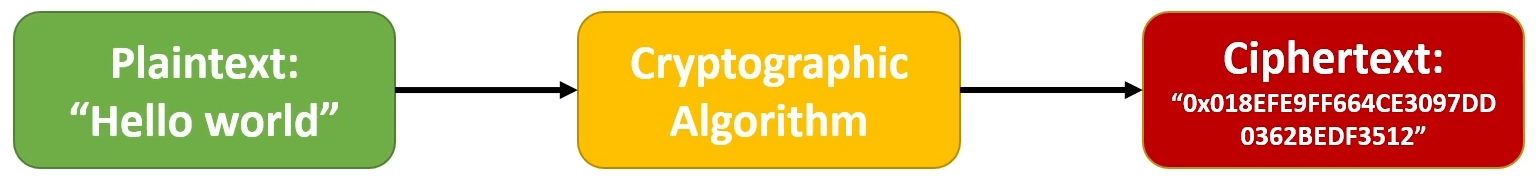
\includegraphics[width=\linewidth,keepaspectratio]{images/lecture05/encryption-flow.png}

\begin{thm}[title=Core requirement: Invertibility]
    \[ \forall K, M,\ D_K(E_K(M)) = M \]
    If not, Bob cannot recover the original message $M$.\\
    \textbf{Security requirement:} these functions must also be \textbf{hard to invert} \textit{without} knowing the key $K$.
\end{thm}

\begin{defn}[title=Types of adversaries]
    Security is always measured relative to the power of the \textbf{adversary (Eve)}.
    \begin{itemize}
        \item \textbf{Passive eavesdropper:} Eve can only \textit{read} the ciphertext.
        \item \textbf{More active attacker:} Eve can influence the system, e.g. convince Alice to send Bob specific messages, observe the precise time Bob takes to run his algorithm\ldots{} anything beyond just observing communication.
    \end{itemize}
\end{defn}

\begin{defn}[title=Active model 1: Known Plaintext Attack (KPA)]
    \begin{itemize}
        \item \textbf{Scenario:} Eve has access to multiple pairs $(M, C)$ of messages and their ciphertexts, all encrypted with the secret key $K$.
        \item \textbf{Goal:} from these pairs, guess the key $K$ to decrypt other messages.
    \end{itemize}
    \textit{Substitution cipher:} if $M$ = ``THE QUICK BROWN FOX'' is known, Eve recovers many letter mappings at once, no frequency analysis needed.
\end{defn}

\begin{defn}[title=Active model 2: Chosen Plaintext Attack (CPA)]
    \begin{itemize}
        \item \textbf{Scenario:} Eve can convince Alice (or the system) to encrypt arbitrary messages \textit{chosen by Eve} with the secret key.
        \item \textbf{More abstractly:} for any chosen plaintext $m$, Eve can get $E_K(m)$.
    \end{itemize}
    Eve is assumed to have access to an \textbf{encryption oracle}.
\end{defn}

\begin{defn}[title=Practical threat model: Side-channel attacks]
    \begin{itemize}
        \item \textbf{Scenario:} Eve can access an ideal oracle, but also measure physical characteristics of the actual implementation while it is encrypting/decrypting.
        \item \textbf{Timing attack:} Eve measures \textbf{how long} it takes to encrypt and decrypt.
        \item \textbf{Power analysis:} Eve observes the \textbf{energy consumed} by the device (e.g., a credit card) doing the crypto.
    \end{itemize}
    \textit{Realistic:} you own a device (phone, smart card, chip) holding another party's keys (bank, Google) that should stay unreadable to you.
\end{defn}

\begin{thm}[title=Perfect secrecy]
    $\forall m, c,\ \PR(M = m \mid E_K(M) = c) = \PR(M = m)$
\end{thm}

\begin{defn}[title=One-time pad (OTP)]
    $K$: \textbf{random} bits, \textbf{as long as} $m$, pre-shared.
    \[ \mathrm{Enc}(k, m) = m \oplus k \qquad \mathrm{Dec}(k, c) = c \oplus k \]
    \textbf{Perfectly secret}: $K$ and $m$ are independant.
\end{defn}

\begin{warn}[title=The key problem of OTP]
    The key must be \textbf{truly random}, \textbf{message-length} and \textbf{used only once}.
\end{warn}

\begin{defn}[title=Two main types of symmetric schemes]
    Encryption and decryption use \textbf{the same key}.
    \begin{itemize}
        \item \textbf{Block ciphers:} operate on fixed-size blocks (e.g., 128 bits).
        \item \textbf{Stream ciphers:} operate one bit/byte at a time.
    \end{itemize}
\end{defn}

\begin{defn}[title=Stream ciphers: the pseudo-OTP]
    Like the OTP, but the random pad is replaced by a \textbf{pseudo-random} stream generated from a short key.
    \par\vspace{1pt}{\centering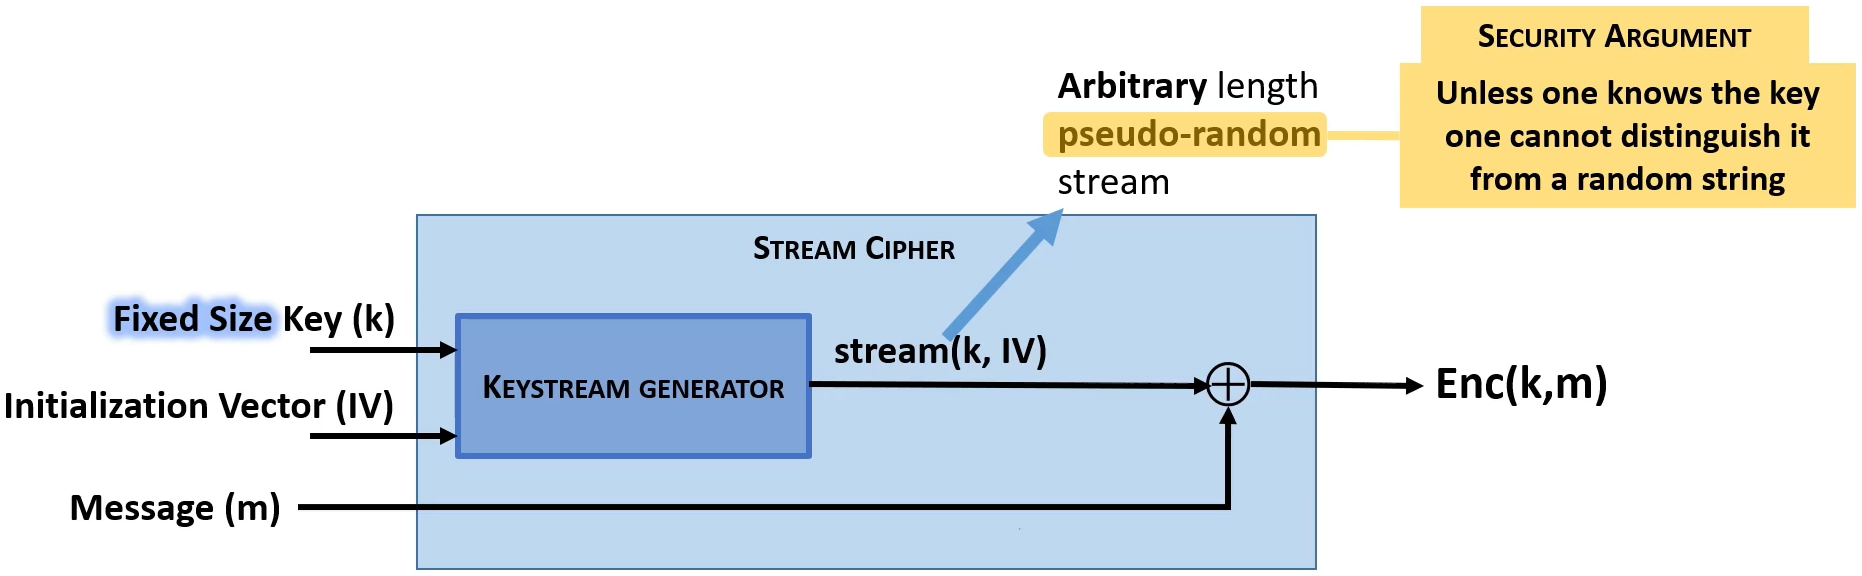
\includegraphics[width=\linewidth,keepaspectratio]{images/lecture05/stream-cipher.png}\par}\vspace{1pt}
    Initialization vector \textit{IV:} \textbf{public}, fresh per message, so the same $K$ never repeats $S$.
\end{defn}

\begin{warn}[title=Cryptanalysis: the problem with periodicity]
    \textbf{Finite state} $\Rightarrow$ eventually \textbf{periodic}: if the message is longer than the period, the stream \textit{repeats}.\\
    \textbf{Attack:} period found and too small $\Rightarrow$ whole key stream known.
\end{warn}

\begin{thm}[title=Diffie-Hellman key exchange]
    Public: prime $p$ and generator $g$.
    \begin{itemize}
        \item \textbf{Alice:} secret $a$, sends $A = g^a \bmod p$.
        \item \textbf{Bob:} secret $b$, sends $B = g^b \bmod p$.
    \end{itemize}
    \[ K = B^a = A^b = g^{ab} \pmod p \]
\end{thm}

\begin{warn}[title=DH: man-in-the-middle (MITM)]
    Eve intercepts $A$ and $B$ and sends her own value to each side: Alice gets the key $K_{AE}$ with Eve, Bob gets $K_{BE}$ with Eve.\\
    Eve can \textbf{read, modify and relay} everything. DH gives key \textbf{agreement}, not \textbf{authentication}: secure against a \textit{passive} Eve only.
\end{warn}

\begin{defn}[title=The need for trust (authentication)]
    DH solves \textbf{key distribution}, but creates the \textbf{identity verification problem}.
    \begin{itemize}
        \item \textbf{Solution:} pair DH with a mechanism like \textbf{digital signatures} to verify identity (next week).
        \item \textbf{Setup:} parties still need to trust a third party (a \textbf{Certificate Authority}) for public key ownership.
    \end{itemize}
\end{defn}

\section{Lecture 6 - Applied Cryptography II}

\begin{defn}[title=Integrity]
    Infos cannot be modified by \textbf{unauthorized parties}.
\end{defn}

\begin{defn}[title={Authentication (digital signature)}]
    \begin{itemize}
        \item Bob signs with his \textbf{Secret Signing Key}.
        \item Alice decrypts with her \textbf{Secret Encryption Key}, then verifies the signature with Bob's \textbf{\mbox{Verification} Public Key}.
        \item \textit{Asymmetric:} different keys sign and verify.
    \end{itemize}
    $\checkmark$ $\Rightarrow$ authenticity, integrity, non-repudiation.
\end{defn}

{\centering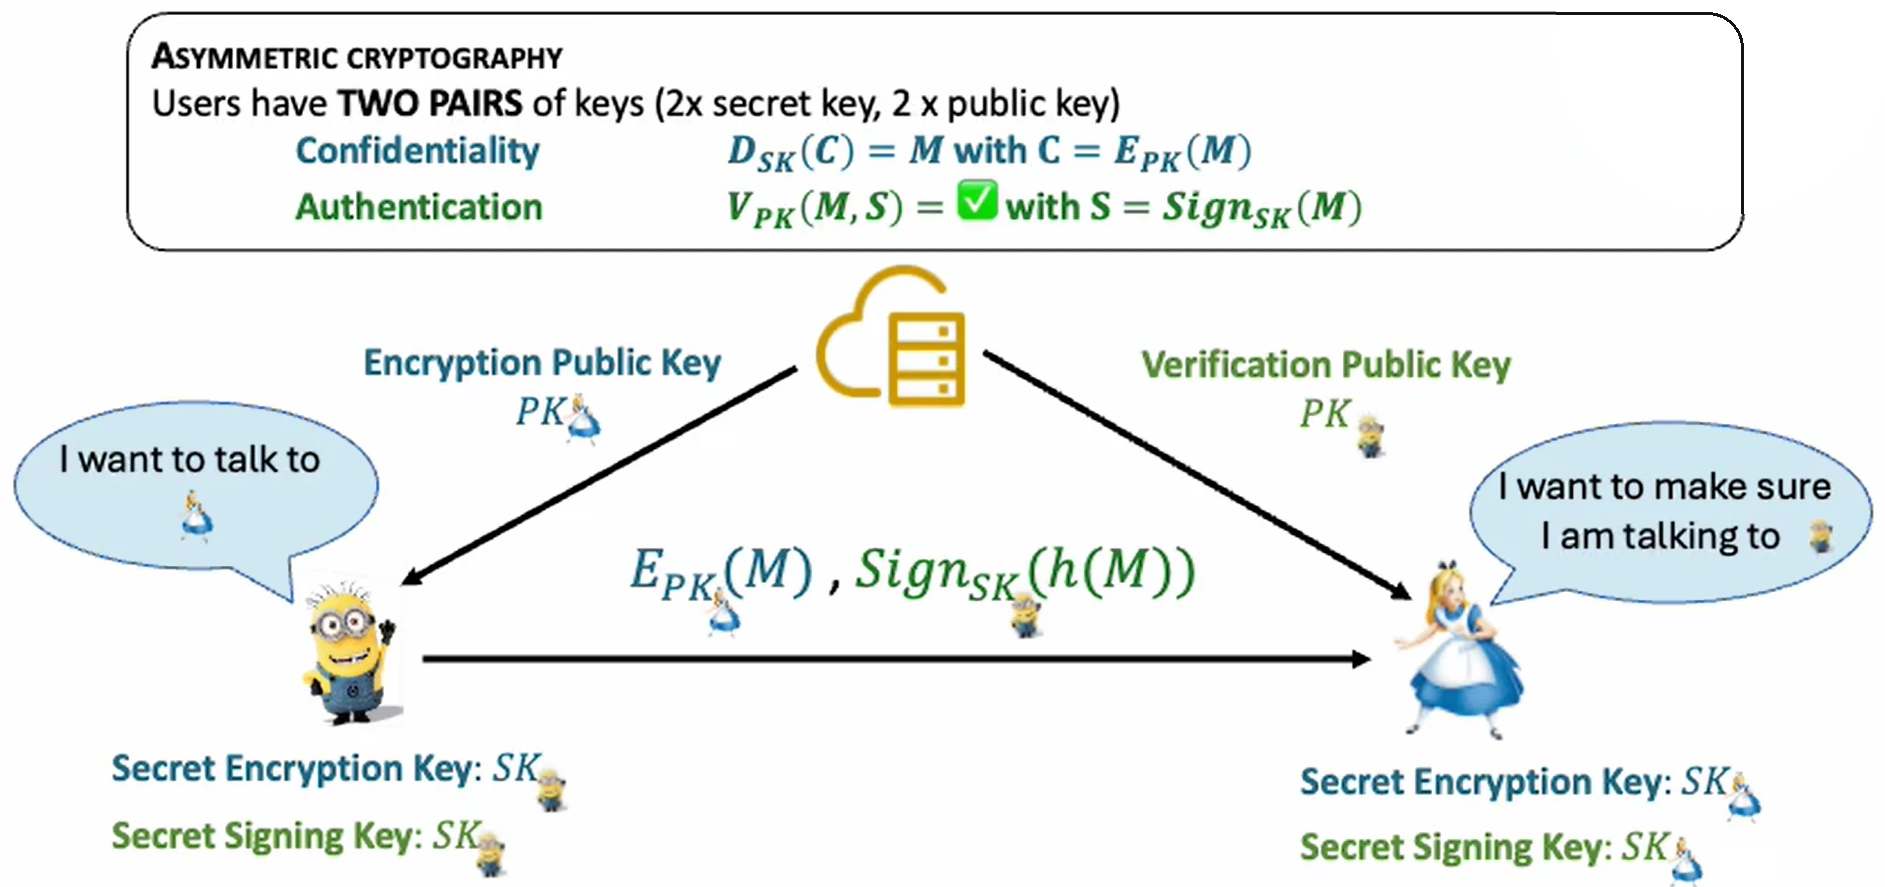
\includegraphics[width=\linewidth,keepaspectratio]{images/lecture06/all-together.png}\par}

\begin{defn}[title=Block cipher modes of operation]
    Blocks are the size of the key (128/256 bits) but messages are longer: iterate.
    \begin{itemize}
        \item \textbf{ECB (Electronic Code Book):} $C_i = E_K(M_i)$. $M_i = M_j \Rightarrow C_i = C_j$: leaks information.
        \item \textbf{CBC (Cipher Block Chaining):} $C_0 = IV$, $C_i = E_K(M_i \oplus C_{i-1})$. Random-looking, but errors propagate and no single-block decryption.
        \item \textbf{CTR (Counter):} $C_i = M_i \oplus E_K(\mathrm{Nonce} + i)$. Blocks independent: parallel, and no $D_K$ needed.
    \end{itemize}
\end{defn}

\begin{warn}[title=Block ciphers: strengths and weaknesses]
    \begin{itemize}
        \item[$+$] \textbf{High diffusion:} one symbol spreads into several.
        \item[$+$] \textbf{Immunity to tampering:} hard to insert symbols undetected.
        \item[$-$] \textbf{Potentially slow:} a whole block is needed first.
        \item[$-$] \textbf{Error propagation} in some modes.
    \end{itemize}
\end{warn}

\begin{defn}[title=Message Authentication Code (MAC)]
    Encryption alone gives no integrity: Eve changes $C$ and Bob decrypts a different $M$. Symmetric fix:
    \par{\centering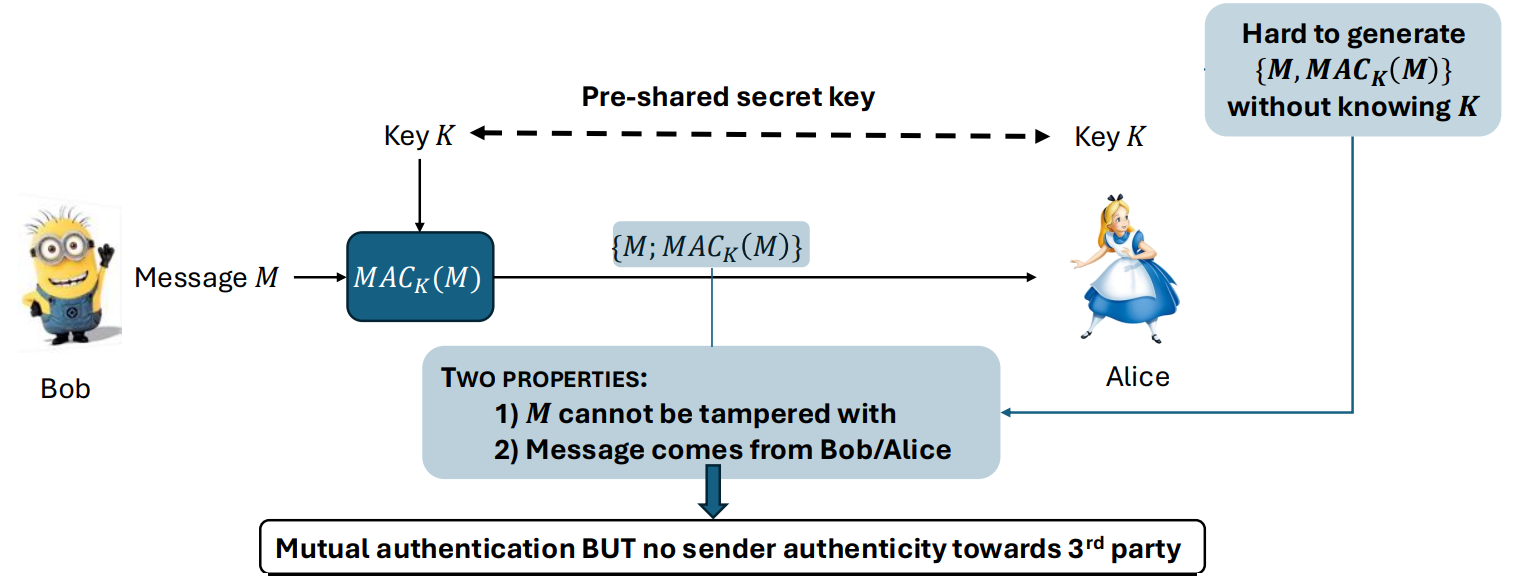
\includegraphics[width=\linewidth,keepaspectratio]{images/lecture06/mac.png}\par}
    \textbf{CBC-MAC:} $C_0 = 0$, $C_i = E_K(M_i \oplus C_{i-1})$, MAC $= $ last block. Deterministic, secure only if the length of $M$ is known.
\end{defn}

\begin{defn}[title=Confidentiality + integrity (symmetric)]
    \begin{itemize}
        \item \textbf{Encrypt-and-MAC:} no integrity on $C$, integrity on $M$, leaks.
        \item \textbf{MAC-then-encrypt:} no integrity on $C$, integrity on $M$, no leaks.
        \item \textbf{Encrypt-then-MAC (use this one):} integrity on $C$, integrity on $M$, no leaks.
    \end{itemize}
\end{defn}

\iffalse
\section{Lecture 5 - Network \& File Syscalls}

\begin{defn}[title=Permission bits]
    Am I the \textbf{owner}? → use USR bits.\\
    Am I in the \textbf{group}? → use GRP bits.\\
    Otherwise → use OTH bits.\\
    \textit{Only the first matching category applies — even if another gives more rights.}
\end{defn}

\begin{prop}[title=Syscall success conditions]
    \begin{tabular}{ll}
        \texttt{open(O\_RDONLY)} & \texttt{r} on file \\
        \texttt{open(O\_WRONLY)} & \texttt{w} on file \\
        \texttt{open(O\_RDWR)}   & \texttt{r}+\texttt{w} on file \\
        \texttt{open(O\_CREAT)}  & \texttt{w}+\texttt{x} on dir \\
        \texttt{read(fd,...)}    & fd open, mode=read \\
        \texttt{write(fd,...)}   & fd open, mode=write \\
        \texttt{close(fd)}       & fd open \\
    \end{tabular}

    \textbf{Every dir} in the path needs \texttt{x} to be traversed.\\
    Any syscall on a \textbf{closed} fd fails immediately.
\end{prop}

\begin{thm}[title=\texttt{S\_*} flags]
    Only used with \texttt{O\_CREAT} to set the new file's permissions. \textbf{Ignored} otherwise.
\end{thm}

\section{Lecture 8 - Forwarding and IP}

Forwarded using the \textbf{longest matching prefix}.

\begin{defn}[title=Broadcast IP address (+1)]
The \texttt{biggest IP address} an IP subnet. If a packet has this destination, it's destined to \textbf{all the end-systems} and \textbf{routers} in the IP subnet.
\end{defn}

\begin{prop}[title=Global reachability]
    Every end-system must be reachable from any other end-system.
\end{prop}
 
\begin{thm}[title=NAT: Layering violation (but it works)]
    A router becomes a NAT only when it's configured to translate between private and public addresses.
    \begin{itemize}
        \item Requires \textbf{per-connection state} at the border routers of the private IP subnets.
        \item An end-system inside a private IP subnet is \textbf{unreachable} from the outside world. [trick possible]
    \end{itemize}
\end{thm}

\section{Lecture 9 - Routing \& BGP}

\begin{prop}[title=Dijkstra's (Link state: converges faster)]
    \begin{enumerate}
        \item At each step, consider a new router starting from "closest" neighbor
        \item Check whether current paths can be improved
        \item End when no improvement is possible
    \end{enumerate}
\end{prop}
\begin{prop}[title=Bellman-Ford (Distance vector: less bandwitdh)]
    \begin{enumerate}
        \item All neighbors exchange information
        \item Each router checks whether it can improve current paths by leveraging the new information
        \item End when no improvement is possible
    \end{enumerate}
\end{prop}

\begin{thm}[title=Internet rounting challenges]
    \begin{itemize}
        \item \textbf{Admin:} An ISP may want to hide its link costs
        \item \textbf{Scale:} Too many IP subnets may cause trouble
    \end{itemize}
\end{thm}

\begin{prop}[title=Border Gateway Protocol (BGP)]
    Inter-AS Routing : Not always the SP. Bellman
    \begin{enumerate}
        \item All neighbors exchange reachable prefixes
        \item Each router checks whether it can improve paths
        \item End when no improvement is possible
    \end{enumerate}
\end{prop}

\begin{thm}[title=Internet rounting solutions]
    \begin{itemize}
        \item Router $\leftrightarrow$ with \textbf{local} router
        \item Border router $\leftrightarrow$ with \textbf{external neighbor}
        \item Router keeps \textbf{forwarding state} for (1) \textbf{local IP subnets} and (2) \textbf{foreign aggregate IP prefixe}
    \end{itemize}
\end{thm}

\section{Lecture 10 - Link layer \& Ethernet}

\begin{defn}[title=Address Resolution Protocol (ARP)]
    Resolves an IP address to a MAC address (to build the L2 frame) via \textit{broadcast} + \textit{caching}.\\
    Naïve broadcast may cause forwarding loops $\Rightarrow$ use a \textbf{spanning tree} to eliminate cycles.
\end{defn}

\section{Lecture 11 - File Systems}

\begin{thm}[title=Persistence]
    State that \textbf{outlives the process that created it} (unlike DRAM, which is volatile).
\end{thm}

\begin{prop}[title=File System]
    Abstracts persistent blocks into: \textbf{Name}, \textbf{Organize}, \textbf{Share}, \textbf{Protect}. Built on \textbf{files} and \textbf{directories}.
\end{prop}

\begin{defn}[title=File]
    Named array of bytes (untyped) with \textbf{data} + \textbf{metadata} (size, owner, permissions, \ldots).
\end{defn}

\begin{defn}[title=Inode]
    Fixed-size on-disk record — one per file: \textbf{metadata} + \textbf{pointers to data blocks}.
\end{defn}

\begin{defn}[title=Inode Table]
    Fixed array indexed by inode number.
\end{defn}

\begin{defn}[title=Directory (special file)]
    Array of \textbf{\{filename, inode\}} pairs per partition
\end{defn}

\begin{defn}[title=File Descriptor Table]
    Per-process. fd $\to$ (\textbf{inode}, \textbf{mode}, \textbf{offset}). \quad \textbf{0}=\texttt{STDIN}, \textbf{1}=\texttt{STDOUT}, \textbf{2}=\texttt{STDERR}.
\end{defn}

\section{Lecture 12 - Processes and Threads}

\begin{defn}[title=Process]
    An instance of a running program. Has its own \textbf{isolated memory space} (code, data, heap, stack) and OS resources (file descriptors, etc.).
\end{defn}

\begin{defn}[title=Thread]
    A unit of execution \textbf{within} a process. Threads share the process's memory and resources, but each has its own \textbf{stack} and \textbf{program counter}.
\end{defn}

\begin{thm}[title=Key properties]
    \begin{itemize}
        \item \textbf{Identifier}: unique id for processes and threads
        \item Each Thread/Process has the \textbf{illusion} that is it the only one occupying the CPU/Memory (resp.)
    \end{itemize}
\end{thm}

\section{Lecture 13 - Sharing the CPU}

\begin{prop}[title=CPU mode \& instructions]
    CPU stores a privilege level: \textbf{Kernel mode} (high) or \textbf{User mode} (low).
    \begin{itemize}
        \item \textbf{Non-privileged:} executable anytime
        \item \textbf{Privileged:} only in kernel mode
    \end{itemize}
\end{prop}

\begin{thm}[title=Limited direct execution (invoking the kernel)]
    Syscall / Exception / Interrupt
\end{thm}

\begin{prop}[title=Process lifecycle]
    \begin{itemize}
        \item \texttt{fork}: creates a \textbf{child} process (copy of parent)
        \item \texttt{exec}: replaces process image with a new program
        \item \texttt{exit}: terminates the process
        \item \texttt{wait}: parent waits for child to finish
    \end{itemize}
\end{prop}

\begin{prop}[title=Type of system processes]
    \begin{itemize}
        \item \textbf{Init}: first process after boot
        \item \textbf{Idle}: runs when nothing else can
        \item \textbf{Shell}: spawns new process on command
        \item \textbf{GUI manager}: spawns new process on click
    \end{itemize}
\end{prop}

\section{Lecture 14 - Memory \& Loose Ends}

\begin{prop}[title=End of a process]
    \texttt{exit()} syscall: kernel destroys memory image but \textbf{keeps exit status} $\Rightarrow$ process becomes a \textbf{zombie} until parent \textbf{reaps} it via \texttt{wait()} to read the exit status.
\end{prop}

\section{Lecture 15 - CPU Scheduling}

\begin{defn}[title=Scheduling Metrics]
    \textbf{Turnaround time} = completion - arrival. \\\textbf{Response time} = first run - arrival.
\end{defn}

\begin{defn}[title=FIFO]
    Run jobs in arrival order. Suffers from \textbf{convoy effect}: short jobs stuck behind long ones.
\end{defn}

\begin{defn}[title=SJF (Shortest Job First)]
    Run shortest job first. Optimal turnaround if all jobs arrive simultaneously. Non-preemptive.
\end{defn}

\begin{defn}[title=STCF (Shortest Time-to-Completion First)]
    Preemptive SJF: preempt if a new job has less remaining time. Optimal turnaround.
\end{defn}

\begin{defn}[title=Round Robin (RR)]
    Each job runs for a fixed \textbf{quantum}, then preempted. Good response time, poor turnaround.
\end{defn}

\begin{warn}[title=Tradeoff]
    SJF/STCF optimizes \textbf{turnaround}. RR optimizes \textbf{response time}. Hard to do both.
\end{warn}

\begin{defn}[title=MLFQ (Multi-Level Feedback Queue)]
    Multiple queues; lower priority = longer time slice.
    \begin{itemize}
        \item \textbf{R1:} priority(A) $>$ priority(B) $\Rightarrow$ A runs
        \item \textbf{R2:} priority(A) $=$ priority(B) $\Rightarrow$ RR
        \item \textbf{R3:} new job starts at \textbf{top} priority
        \item \textbf{R4:} uses full slice $\Rightarrow$ \textbf{demoted}; blocks early $\Rightarrow$ \textbf{keeps} priority
        \item \textbf{R5:} periodically move all jobs to top (\textbf{priority boost}) — avoids starvation
    \end{itemize}
\end{defn}

\section{Lecture 17/18 - Concurrency}
\textbf{Concurrency:} how should we manage tasks\\
\textbf{Parallism:} how to execute tasks in parallel

\begin{defn}[title=Race condition \& Data race]
    \begin{itemize}
        \item \textbf{Race cond.:} behavior depends on thread timing
        \item \textbf{Data race:} unsynchronized concurrent access to shared writable state
    \end{itemize}
\end{defn}

\begin{defn}[title=Critical section]
    Code that will be executed by the threads. Must enforce: \textbf{atomicity} (uninterruptible) and \textbf{mutual exclusion} (one thread at a time).
\end{defn}

\begin{warn}[title=Synchronization primitives]
    \begin{itemize}
        \item \textbf{Lock} $\rightarrow$ prevent concurrent access
        \item \textbf{Condition var.} $\rightarrow$ wait until a condition holds
        \item \textbf{Semaphore} $\rightarrow$ count available resources
    \end{itemize}
\end{warn}


\end{multicols*}
\begin{multicols*}{3}

{\centering\includegraphics[width=\linewidth,keepaspectratio]{images/net_stack.png}\par}
{\centering\includegraphics[width=\linewidth,keepaspectratio]{images/io_stack.png}\par}
{\centering\includegraphics[width=\linewidth,keepaspectratio]{images/lecture05/ls-l-entry-anatomy.png}\par}

\begin{prop}[title=\texttt{open()} flags / permission mode]
    \begin{tabular}{ll}
        \texttt{O\_CREAT}  & create file if it doesn't exist \\
        \texttt{O\_EXCL}   & fail if file already exists \\
        \texttt{O\_APPEND} & always write at end of file \\
        \texttt{O\_TRUNC}  & truncate file on open \\
        \texttt{O\_RDONLY} & read only \\
        \texttt{O\_WRONLY} & write only \\
        \hline
        \texttt{S\_IRUSR} & read by owner \\
        \texttt{S\_IWUSR} & write by owner \\
        \texttt{S\_IXUSR} & execute by owner \\
        \texttt{S\_IRGRP} & read by group \\
        \texttt{S\_IROTH} & read by others \\
        \texttt{0}        & no permissions \\
    \end{tabular}
\end{prop}

\begin{lstlisting}
INIT-SINGLE-SOURCE(G, s)
    s.d = 0
    for v in G.V: v.d = inf; v.pi = NIL

RELAX(u, v, w)
    if v.d > u.d + w(u, v)
        v.d = u.d + w(u, v); v.pi = u

BELLMAN-FORD(G, w, s)
    INIT-SINGLE-SOURCE(G, s)
    for i = 1 to |G.V| - 1
        for (u, v) in G.E: 
            RELAX(u, v, w)

DIJKSTRA(G, w, s)
    INIT-SINGLE-SOURCE(G, s)
    S = {}
    Q = G.V   // min-priority queue (sorted by d(v))
    while Q != {}:
        u = EXTRACT-MIN(Q)
        S = S U {u}
        for each vertex v in G.Adj[u]:
            RELAX(u, v, w)
\end{lstlisting}

{\centering\includegraphics[width=0.8\linewidth,keepaspectratio]{images/bellman_example.png}\par}
{\centering\includegraphics[width=\linewidth,keepaspectratio]{images/dijkstra_example.png}\par}

\begin{defn}[title=Powers of ten]
    \begin{itemize}
        \item 1 KB (kilobyte) $= 10^3 = 1\,000$ bytes
        \item 1 MB (megabyte) $= 10^6 = 1\,000\,000$ bytes
        \item 1 GB (gigabyte) $= 10^9 = 1\,000\,000\,000$ bytes
    \end{itemize}
\end{defn}

\begin{defn}[title=Powers of two]
    \begin{itemize}
        \item 1 KiB (kibibyte) $= 2^{10} = 1\,024$ bytes
        \item 1 MiB (mebibyte) $= 2^{20} = 1\,048\,576$ bytes
        \item 1 GiB (gibibyte) $= 2^{30} = 1\,073\,741\,824$ bytes
    \end{itemize}
\end{defn}

\subsection{Process state diagram}
{\centering\includegraphics[width=0.6\linewidth,keepaspectratio]{images/lecture14/process_fsm.png}\par}

\subsection{Thread state diagram}
{\centering\includegraphics[width=0.6\linewidth,keepaspectratio]{images/lecture14/thread_fsm.png}\par}

{\centering\includegraphics[width=\linewidth,keepaspectratio]{images/tahoe_reno.png}\par}
{\centering\includegraphics[width=0.8\linewidth,keepaspectratio]{images/reno_example.png}\par}

{\centering\includegraphics[width=\linewidth,keepaspectratio]{images/multi-level-indexing.png}\par}


{\centering\includegraphics[width=\linewidth,keepaspectratio]{images/lecture13/kernel_overview.png}\par}

{\centering\includegraphics[width=\linewidth,keepaspectratio]{images/partition.png}\par}
{\centering\includegraphics[width=\linewidth,keepaspectratio]{images/read_write_on_disk.png}\par}

\newcolumn

\begin{small}
\noindent\textbf{Web and DNS}\\
All web client processes keep caches with the most recently retrieved web objects. All DNS client and DNS server processes keep caches with the most recently retrieved DNS records (e.g., DNS name $\to$ IP address mappings). If the TTL of a retrieved web object or DNS record is not explicitly stated, assume that it is 1 hour. Web processes communicate over TCP. DNS processes communicate over UDP.

\noindent\textbf{TCP}\\
When a TCP-related question does not mention the receiver window at all, assume that the receiver window is very large and it does not affect the rate at which data is exchanged. When you are given a scenario where Processes A and B exchange data over TCP, assume that they use the same TCP connection for all the data, unless you are explicitly told otherwise. When you are given a scenario where client Process A establishes a TCP connection with server Process B and A sends a request to B; assume that the second segment sent by A to B already carries bytes of data and has SEQ number 1. When computing the amount of time it takes for a data segment to go from Alice to Bob plus the time it takes for an ACK to go from Bob to Alice, when there is no other traffic present (so, no queuing delays): Do take into account the transmission delay experienced by the data segment, but not for the ACK.

\noindent\textbf{Packet Switch Behavior}\\
All packet switches are store-and-forward packet switches. All packet switches have infinite queues. All packet switches introduce 0 processing delays. All packet switches behave as follows: There is always one queue per link and it stores packets that are going out that link. When a packet arrives, the switch immediately examines the packet, determines the correct outgoing link, and stores the packet in the queue that feeds that link. If two packets arrive at a switch and are put in the same queue at the same time, the order in which they are put in the queue is random. Assume the order that makes the solution simpler. All queues are served following a FIFO (first in first out) policy.

\noindent\textbf{Insignificant Headers \& Transmission delays}\\
If a problem tells you that ``lower-layer headers are insignificant'': If you need to compute the transmission delay of a packet, and that packet does not carry any application-layer content (e.g., it is a TCP segment that carries an ACK but no data), then this packet experiences transmission delay 0.

\noindent\textbf{IP subnets \& prefixes}\\
Each network interface of a router has an IP address (and, of course, a MAC address). Network interfaces of L2 switches have no IP or MAC addresses. Each IP subnet has a broadcast IP address (which is the highest IP address in the subnet), but NO network IP address. Each end-system knows the IP address of its default gateway.

\noindent\textbf{File access}\\
We don't expect you to reason about bitmap accesses. We do expect you to reason about inode and data block accesses. Reading a file does not trigger a write to the file's inode to update the read access time. Closing a file does not trigger any block access. There exists a file system (FS) cache (which is the same thing as a block cache), unless you are explicitly told that it does not exist. The FS/block cache has infinite size unless you are explicitly told otherwise. The FS/block cache is write-through. I.e., when a process makes a write syscall to write N bytes to disk, this causes the FS/block cache to be updated, but it also triggers as many block accesses as necessary to write the N bytes to disk (and to update the inode of the file that's being written). Differently said: The presence of the FS/block cache may remove the need for some read block accesses, but it cannot remove the need for write block accesses.

\noindent\textbf{Scheduling}\\
If a thread terminates or blocks after running for a fraction of a time tick (e.g., after 0.99 time ticks), assume that ``nothing'' happens during the rest of the current time tick. Differently said: Assume that the OS scheduler can only run at integer time-tick values, e.g., time tick 0, time tick 1, etc.
\end{small}
\fi

\end{multicols*}
\end{document}
